\begin{figure}[p]
\vspace{-0.03\textwidth}
\hspace{-0.1\textwidth}
\begin{minipage}{0.32\textwidth}
% Does not work in newer versions of pdflatex -- runs out of memory.
%\lstinputlisting[style=pydiffsmall, backgroundcolor=\color{backcolour}]{code/diff_full.diff}
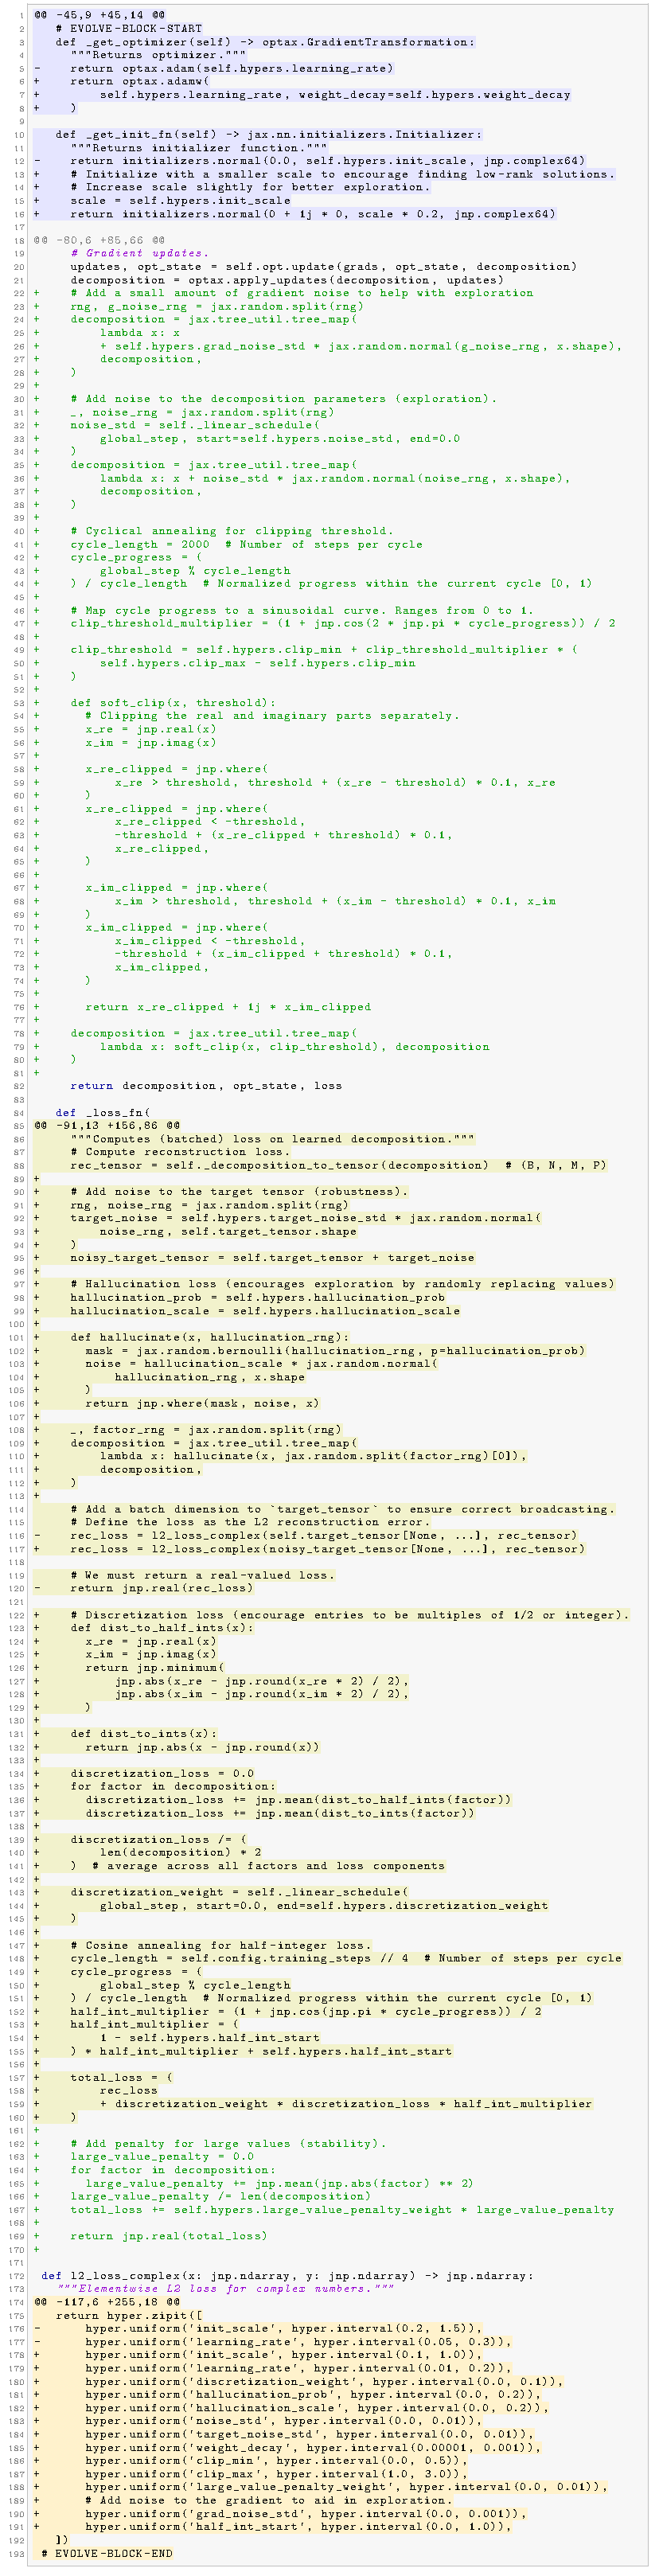
\includegraphics[width=\linewidth]{code/diff_full.pdf}
\end{minipage}
\hspace{0.06\textwidth}
\begin{minipage}{0.59\textwidth}%
\lstinputlisting[style=pydiffmedium, backgroundcolor=\color{highlightblue}]{code/zoom1.diff}
\vspace{-0.4em}
\lstinputlisting[style=pydiffmedium, backgroundcolor=\color{highlightyellow}]{code/zoom2.diff}
\vspace{-0.4em}
\lstinputlisting[style=pydiffmedium, backgroundcolor=\color{highlightorange}]{code/zoom3.diff}
\end{minipage}
\hspace{-0.1\textwidth}
\caption{Changes proposed by \method to discover faster matrix multiplication algorithms. The full diff is outlined on the left (see magnified version in~\Cref{fig:relaxed-opt-diff-appendix-1,fig:relaxed-opt-diff-appendix-2,fig:relaxed-opt-diff-appendix-3}) and some excerpts are highlighted on the right. In this example, \method proposes extensive changes across several components, including the optimizer and weight initialization (top right), the loss function (middle right), and hyperparameter sweep (bottom right). These changes are highly non-trivial, requiring 15 mutations during the evolutionary process.}\label{fig:relaxed-opt-diff}
\centering
\end{figure}
